\documentclass{beamer}
\usetheme{focus}

\title{\centering Fearless concurrency \\ ~}
\subtitle{ or how can the compiler save us?}
\author{\centering ~ \\ A paper presentation about uniqueness and reference immutability \\ ~}
\titlegraphic{}%
\institute{Thomas Lacroix \\ KTH -- Pardis 18}
\date{25 09 2018}

%%%

\usepackage{listings}
\usepackage{color}

\definecolor{dkgreen}{rgb}{0,0.6,0}
\definecolor{gray}{rgb}{0.5,0.5,0.5}
\definecolor{mauve}{rgb}{0.58,0,0.82}

\lstset{frame=tb,
  language=Java,
  aboveskip=3mm,
  belowskip=3mm,
  showstringspaces=false,
  columns=flexible,
  basicstyle=\ttfamily\scriptsize,
%  basicstyle={\small\ttfamily},
  numbers=left,
  numberstyle=\tiny\color{gray},
  keywordstyle=\color{blue},
  commentstyle=\color{dkgreen},
  stringstyle=\color{mauve},
  breaklines=true,
  breakatwhitespace=true,
  tabsize=3,
  morekeywords={writable,readable,immutable,isolated}
}


\usepackage{ragged2e}
\apptocmd{\frame}{}{\justifying}{}
\apptocmd{\itemize}{}{\justifying}{}

%%%

\begin{document}

%%%%%%%%%%%%%%%%%%%%%%%%%%%%%%%%%%%%%%%%%%%%%%%%%%%%%%%%%%%%%%%%%%%%%%%%%%%%

\begin{frame}
    \maketitle
\end{frame}

%%%%%%%%%%%%%%%%%%%%%%%%%%%%%%%%%%%%%%%%%%%%%%%%%%%%%%%%%%%%%%%%%%%%%%%%%%%%

\begin{frame}{Main reference}
    \nocite{*}
    \bibliography{bibliography}
    \bibliographystyle{plain}
\end{frame}

%%%%%%%%%%%%%%%%%%%%%%%%%%%%%%%%%%%%%%%%%%%%%%%%%%%%%%%%%%%%%%%%%%%%%%%%%%%%

\begin{frame}{Wanna race with me?}
	\begin{block}{Problem}
	We work for the social care. We would like to sort all the ages of Sweden
	citizens. Can you do that for us?
	\end{block}
	\vfill\pause
	Ok, so there are about 10M people in Sweden.
	\vfill\pause
	\centering
	\newcommand{\blue}{\only<4->{\color{blue}}}
	\newcommand{\green}{\only<5->{\color{dkgreen}}}
	\begin{tabular}{|l|r|}
		\hline
		$ O(\log(N))               $ & $                  20 $ \\
		$ \green O(N)              $ & $ \green   10,000,000 $ \\
		$ \blue O(N \cdot \log(N)) $ & $ \blue   200,000,000 $ \\
		$ O(N^2)                   $ & $ 100,000,000,000,000 $ \\
		\hline
	\end{tabular}
\end{frame}

%%%%%%%%%%%%%%%%%%%%%%%%%%%%%%%%%%%%%%%%%%%%%%%%%%%%%%%%%%%%%%%%%%%%%%%%%%%%

\begin{frame}[fragile]{Wanna race with me?}
	\begin{lstlisting}
class OOneAgeSort implements SortAlgorithm {
    final int MIN_AGE = 0;
    final int MAX_AGE = 300;
    @Override
    public void sort(int[] list) {
        int[] age_count = new int[MAX_AGE-MIN_AGE+1];
        for (int age : list) {
            age_count[age]++;
        }
        int k = 0;
        for (int i = 0; i < age_count.length; i++) {
            for (int j = 0; j < age_count[i]; j++) {
                list[k++] = i;
            }
}   }   }
	\end{lstlisting}
\end{frame}

%%%%%%%%%%%%%%%%%%%%%%%%%%%%%%%%%%%%%%%%%%%%%%%%%%%%%%%%%%%%%%%%%%%%%%%%%%%%

\begin{frame}[fragile]{Wanna race with me?}
	\begin{verbatim}
	{ 4, 10, 5, 2, 10, 4, 6, 7, 8, 7, 8, 4, 10, 11,
	  4, 5, 7, 8, 4, 10, 11, 8, 14 }
	\end{verbatim}
	\centering$\Big\Downarrow$
	\begin{center}
		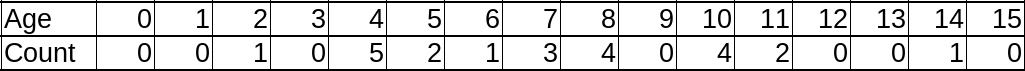
\includegraphics[width=11cm]{img/array-normal.png}
	\end{center}
\end{frame}

%%%%%%%%%%%%%%%%%%%%%%%%%%%%%%%%%%%%%%%%%%%%%%%%%%%%%%%%%%%%%%%%%%%%%%%%%%%%

\begin{frame}{Wanna race with me?}
	\centering Well done!
	\begin{center}
		\frame{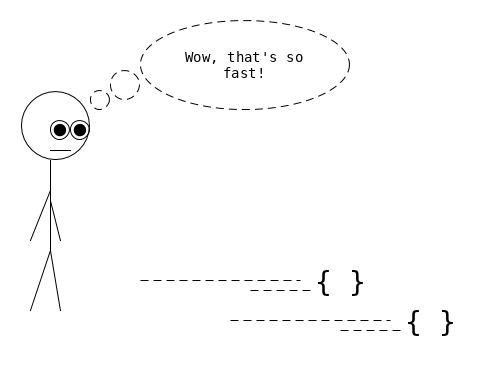
\includegraphics[width=8cm]{uml/amazing-so-fast.png}}
	\end{center}
\end{frame}

%%%%%%%%%%%%%%%%%%%%%%%%%%%%%%%%%%%%%%%%%%%%%%%%%%%%%%%%%%%%%%%%%%%%%%%%%%%%

\begin{frame}{Wanna race with me?}
	\begin{center}
		\frame{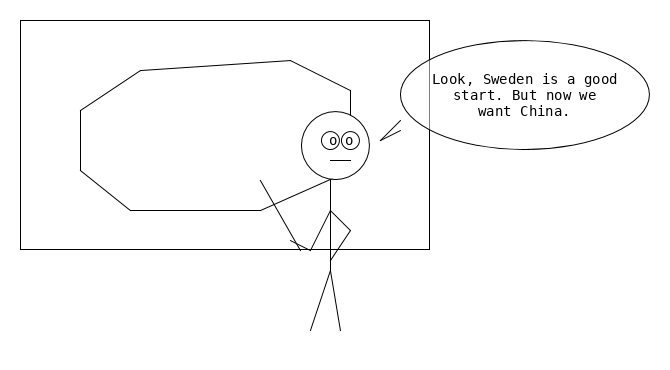
\includegraphics[width=10cm]{uml/want-china-now.png}}
	\end{center}
\end{frame}

%%%%%%%%%%%%%%%%%%%%%%%%%%%%%%%%%%%%%%%%%%%%%%%%%%%%%%%%%%%%%%%%%%%%%%%%%%%%

\begin{frame}{Wanna race with me?}
	\begin{center}
		\frame{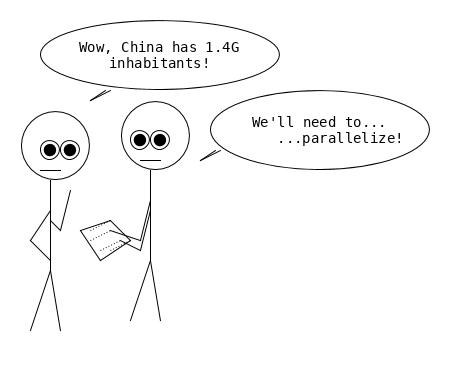
\includegraphics[width=8cm]{uml/china-so-big-need-to-parallelize.png}}
	\end{center}
\end{frame}

%%%%%%%%%%%%%%%%%%%%%%%%%%%%%%%%%%%%%%%%%%%%%%%%%%%%%%%%%%%%%%%%%%%%%%%%%%%%

\begin{frame}[fragile]{Wanna race with me?}
	No problem, we can just split the list and have multiple threads
	go though all the data!
	\begin{lstlisting}
class ParallelLinearAgeSort implements SortAlgorithm {
   public void sort(int[] list) {
      int[] age_count = new int[MAX_AGE-MIN_AGE+1];
      Thread[] ts = new Thread[NUM_THREADS];
      for (int t = 0; t < ts.length; t++) {
         int begin_i = t;
         ts[t] = new Thread(() -> {
            for (int i = begin_i; i < ts.length; i += NUM_THREADS)
               age_count[list[i]]++;
         });
         ts[t].start();
      }
      for (Thread t : ts) t.join();
      // ...
   }
}
	\end{lstlisting}
\end{frame}

%%%%%%%%%%%%%%%%%%%%%%%%%%%%%%%%%%%%%%%%%%%%%%%%%%%%%%%%%%%%%%%%%%%%%%%%%%%%

\begin{frame}{Wanna race with me?}
	\begin{center}
		\frame{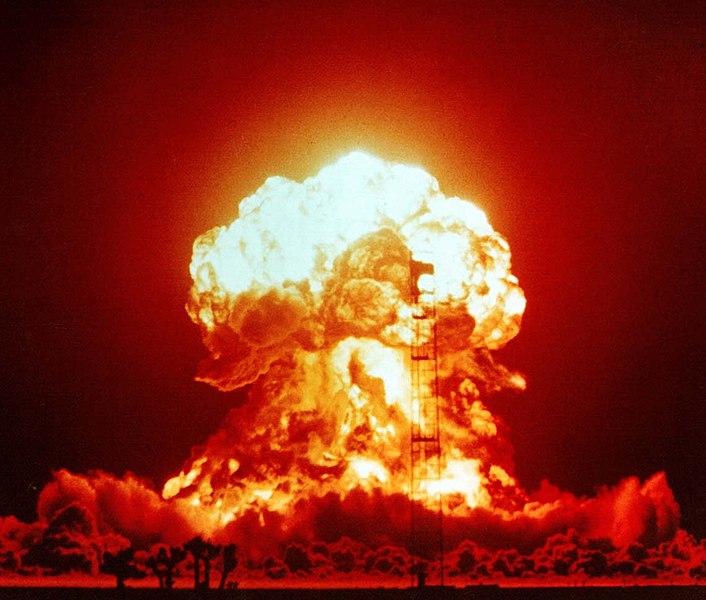
\includegraphics[width=8cm]{img/nuclear.jpg}}
	\end{center}
	\raggedleft
	\tiny{\textit{Photo courtesy of National Nuclear Security Administration
	/ Nevada Site Office [Public domain],\\ via Wikimedia Commons}}
\end{frame}

%%%%%%%%%%%%%%%%%%%%%%%%%%%%%%%%%%%%%%%%%%%%%%%%%%%%%%%%%%%%%%%%%%%%%%%%%%%%

\begin{frame}{Wanna race with me?}
	\begin{center}
		So, what happened?
		\vfill\pause
		$\Rightarrow$ There is a data race.
	\end{center}	
\end{frame}

%%%%%%%%%%%%%%%%%%%%%%%%%%%%%%%%%%%%%%%%%%%%%%%%%%%%%%%%%%%%%%%%%%%%%%%%%%%%

\begin{frame}{Wanna race with me?}
	What is a data race?
	\begin{block}{Definition}
	Data races are defined as:
	\begin{itemize}
		\item two or more threads concurrently accessing a location of memory,
		\item one of them is a write,
		\item one of them is unsynchronized.
	\end{itemize}
	\raggedleft From: Rustonomicon > Races
	\end{block}
	\vfill
\end{frame}

%%%%%%%%%%%%%%%%%%%%%%%%%%%%%%%%%%%%%%%%%%%%%%%%%%%%%%%%%%%%%%%%%%%%%%%%%%%%

\begin{frame}{Wanna race with me?}
	\begin{center}
		\frame{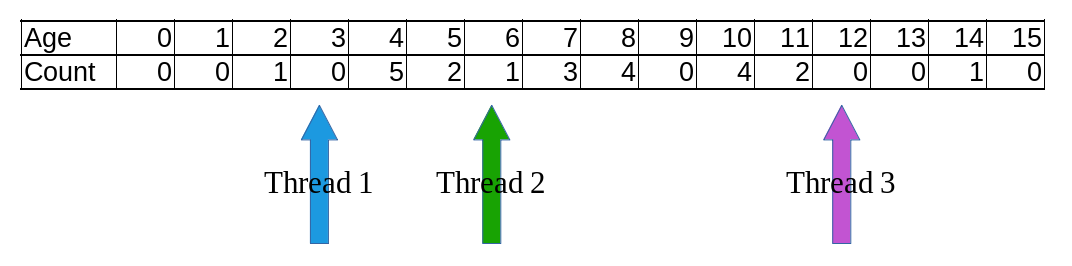
\includegraphics[width=11cm]{img/array-threads-distinct.png}}
		\vfill
		So far so good, the threads operate on distinct cells.
	\end{center}
\end{frame}

%%%%%%%%%%%%%%%%%%%%%%%%%%%%%%%%%%%%%%%%%%%%%%%%%%%%%%%%%%%%%%%%%%%%%%%%%%%%

\begin{frame}{Wanna race with me?}
	\begin{center}
		\frame{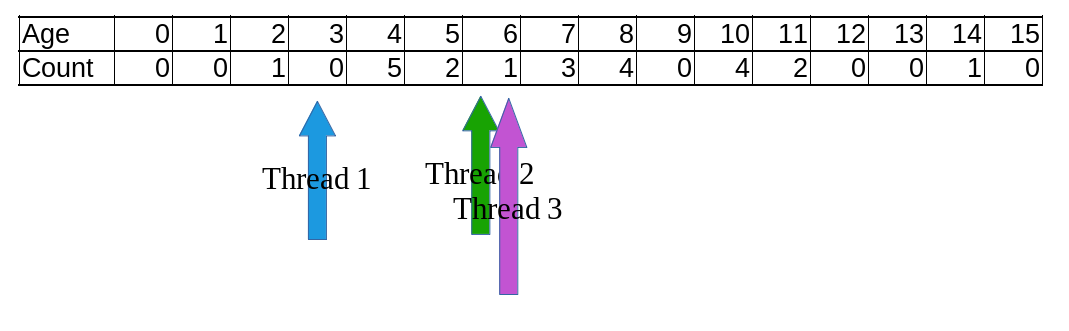
\includegraphics[width=11cm]{img/array-threads-same.png}}
		\vfill
		Oups, they work on the same memory location.
	\end{center}
\end{frame}

%%%%%%%%%%%%%%%%%%%%%%%%%%%%%%%%%%%%%%%%%%%%%%%%%%%%%%%%%%%%%%%%%%%%%%%%%%%%

\begin{frame}{Wanna race with me?}
	\begin{center}
		Could we have seen it right away?\\
		\pause
		Yes.
		\vfill\pause
		Why?\\
		\pause
		$\Rightarrow$ Threads work on the same memory location.
		\vfill\pause
		But that's basic stuff, right?\\
		\pause
		{\color{red} $\Rightarrow$ So, why does that even compile?}
	\end{center}
\end{frame}

%%%%%%%%%%%%%%%%%%%%%%%%%%%%%%%%%%%%%%%%%%%%%%%%%%%%%%%%%%%%%%%%%%%%%%%%%%%%

\begin{frame}{Wanna race with me?}
	Is racy code desirable?
	{\only<2->{\color{red}}Yes} / {\only<2->{\color{dkgreen}}No}.
	\vfill\pause
	Why?
	\pause
	Because it's Undefined Behaviour.\\
	$\Rightarrow$ A compiler can \textbf{forbid} UB.
\end{frame}

%%%%%%%%%%%%%%%%%%%%%%%%%%%%%%%%%%%%%%%%%%%%%%%%%%%%%%%%%%%%%%%%%%%%%%%%%%%%

\section{Compile-time race-freedom\\ guarantee}

%%%%%%%%%%%%%%%%%%%%%%%%%%%%%%%%%%%%%%%%%%%%%%%%%%%%%%%%%%%%%%%%%%%%%%%%%%%%

\begin{frame}{Compile-time race-freedom guarantee}
	\begin{block}{Our problem}
	How can a compiler detect data races?
	\end{block}
	\pause
	\begin{block}{Definition}
	Data races are defined as:
	\begin{itemize}
		\item two or more threads concurrently accessing 
		{\color{blue} the same memory location},
		\item one of them {\color{blue} is a write},
		\item one of them {\color{blue} is unsynchronized}.
	\end{itemize}
	\raggedleft From: Rustonomicon > Races
	\end{block}
\end{frame}
%%%%%%%%%%%%%%%%%%%%%%%%%%%%%%%%%%%%%%%%%%%%%%%%%%%%%%%%%%%%%%%%%%%%%%%%%%%%

\begin{frame}[fragile]{Compile-time race-freedom guarantee}
	\begin{lstlisting}
class ParallelLinearAgeSort implements SortAlgorithm {
   public void sort(int[] list) {
      int[] age_count = new int[MAX_AGE-MIN_AGE+1];
      Thread[] ts = new Thread[NUM_THREADS];
      for (int t = 0; t < ts.length; t++) {
         int begin_i = t;
         ts[t] = new Thread(() -> {
            for (int i = begin_i; i < ts.length; i += NUM_THREADS)
               age_count[list[i]]++;
         });
         ts[t].start();
      }
      for (Thread t : ts) t.join();
      // ...
   }
}
	\end{lstlisting}
	\begin{itemize}
	\item \texttt{age\_count} is accessed by all threads
	\end{itemize}
\end{frame}

%%%%%%%%%%%%%%%%%%%%%%%%%%%%%%%%%%%%%%%%%%%%%%%%%%%%%%%%%%%%%%%%%%%%%%%%%%%%

\begin{frame}{Compile-time race-freedom guarantee}
	\begin{itemize}
	\item \texttt{age\_count} is accessed by all threads
	\end{itemize}
	\vfill
	In other words, {\only<2->{\color{blue}} two threads} share a
	{\only<2->{\color{blue}} writeable reference} on
	{\only<2->{\color{blue}} the same memory location}.
\end{frame}

%%%%%%%%%%%%%%%%%%%%%%%%%%%%%%%%%%%%%%%%%%%%%%%%%%%%%%%%%%%%%%%%%%%%%%%%%%%%

\begin{frame}{Compile-time race-freedom guarantee}
	The paper presents a \textbf{type system} to \textbf{restrict updates}
	to memory to prevent (some) race conditions.\\
	~\\
	They provide a novel combination of \textbf{immutable} and \textbf{unique}
	(isolated) types that ensure \textbf{safe parallelism} (race freedom and
	deterministic execution).
\end{frame}

%%%%%%%%%%%%%%%%%%%%%%%%%%%%%%%%%%%%%%%%%%%%%%%%%%%%%%%%%%%%%%%%%%%%%%%%%%%%

\begin{frame}{Compile-time race-freedom guarantee}
	\newcommand{\bb}{\only<3->{\color{blue}}}
	\newcommand{\bbb}{\only<5->{\color{blue}}}
	
	Reference immutability is based on a set of permission-qualified
	types. The system has four qualifiers:
	\begin{itemize}
	\pause
	\item \textbf{writable:} An ``ordinary'' object reference, which
		  allows {\bb mutation} of its referent.
	\uncover<4->{
	\item \textbf{readable:} A read-only reference, which allows {\bbb no
		  mutation} of its referent. Furthermore, no {\bbb heap traversal}
		  through a read-only reference produces a \texttt{writable}
		  reference (\texttt{writable} references to the same objects
		  {\bbb may exist and be reachable elsewhere}, just not through a
		  \texttt{readable} reference). A readable reference may also
		  refer to an immutable object.
	}
	\end{itemize}
\end{frame}

\begin{frame}{Compile-time race-freedom guarantee}
	\newcommand{\bb}{\only<2->{\color{blue}}}
	
	\begin{itemize}
	\item \textbf{immutable:} A read-only reference which additionally
		  notes that its referent {\bb can never be mutated through any
		  reference}. Immutable references may be aliased by \texttt{readable}
		  or \texttt{immutable} references, but no other kind of reference.
		  All objects reachable from an \texttt{immutable} reference are
		  also \texttt{immutable}.
	\end{itemize}
\end{frame}

\begin{frame}{Compile-time race-freedom guarantee}
	\newcommand{\bb}{\only<2->{\color{blue}}}
	
	\begin{itemize}
	\item \textbf{isolated:} An external reference to an {\bb externally-
		  unique object cluster}. External uniqueness naturally captures
		  {\bb thread locality of data}. An externally-unique aggregate
		  is a cluster of objects that freely reference each other,
	      but for which {\bb only one external reference into the
	  	  aggregate exists}.\\
	  	  All paths to non-immutable objects reachable from the
	  	  isolated reference pass through the isolated reference.
	\end{itemize}
	\texttt{isolated} references must be converted through
	subtyping to another permission before use.
\end{frame}

%%%%%%%%%%%%%%%%%%%%%%%%%%%%%%%%%%%%%%%%%%%%%%%%%%%%%%%%%%%%%%%%%%%%%%%%%%%%

\begin{frame}{Compile-time race-freedom guarantee}
	\begin{center}
		\frame{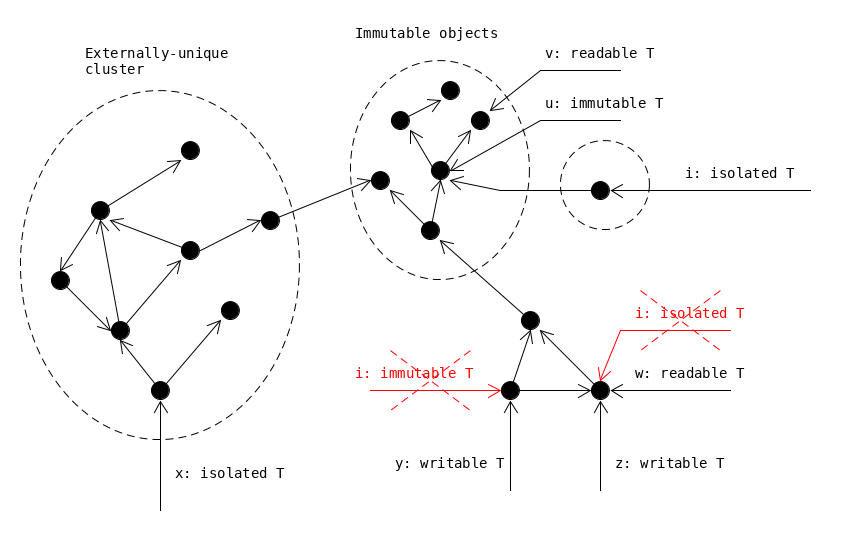
\includegraphics[width=10cm]{uml/writable-readable-immutable-isolated.png}}
	\end{center}
\end{frame}

%%%%%%%%%%%%%%%%%%%%%%%%%%%%%%%%%%%%%%%%%%%%%%%%%%%%%%%%%%%%%%%%%%%%%%%%%%%%

\begin{frame}[fragile]{Compile-time race-freedom guarantee}
	The objective now is to assemble a set of rules to:
	\begin{itemize}
	\item control where modifications can occur
	\item guarantee that modifications cannot occur in some situations
	\end{itemize}
\end{frame}

%%%%%%%%%%%%%%%%%%%%%%%%%%%%%%%%%%%%%%%%%%%%%%%%%%%%%%%%%%%%%%%%%%%%%%%%%%%%

\begin{frame}[fragile]{Compile-time race-freedom guarantee}
	For example, a developer can be sure that a library call to a static
	method with the type signature
	\begin{lstlisting}
		int countElements(readable ElementList lst);
	\end{lstlisting}
	will not modify the list or its elements (through the \texttt{lst}
	reference).	Accessing any field of the argument \texttt{lst} through
	the \texttt{readable} reference passed will produce other \texttt{readable}
	(or \texttt{immutable}) references.
\end{frame}

\begin{frame}[fragile]{Compile-time race-freedom guarantee}
	For example, a developer could not	implement \texttt{countElements()}
	like so:
	\begin{lstlisting}
		int countElements(readable ElementList lst)
		{ lst.head = null; return 0; }
	\end{lstlisting}
	because the compiler would issue a \textbf{type error}. In fact,
	\textbf{any	attempt} within \texttt{countElements()} \textbf{to modify}
	the	list would result in a \textbf{type error}, because \texttt{lst} is
	\textbf{deeply (transitively) read-only}, and writes through read-only
	references are prohibited.
	\vfill
	\textit{This can remind you of the \texttt{const} modifier in C++.}
\end{frame}

%%%%%%%%%%%%%%%%%%%%%%%%%%%%%%%%%%%%%%%%%%%%%%%%%%%%%%%%%%%%%%%%%%%%%%%%%%%%

\begin{frame}[fragile]{Compile-time race-freedom guarantee}
	The \texttt{isolated} permission is a novelty of this work, and
	is particularly important for two reasons.\\
	\pause ~\\
	\textbf{First}, they support natural safe parallelism. Here, threads
	cannot interfere with each other, because they work on distinct memory
	locations.
	\begin{lstlisting}
		isolated IntList l1 = ...;
		isolated IntList l2 = ...;
		{ l1.map(new Incrementor()); }
			|| { l2.map(new Incrementor()); }
	\end{lstlisting}
\end{frame}

%%%%%%%%%%%%%%%%%%%%%%%%%%%%%%%%%%%%%%%%%%%%%%%%%%%%%%%%%%%%%%%%%%%%%%%%%%%%

\begin{frame}[fragile]{Compile-time race-freedom guarantee}
	\textbf{Second}, as the whole object graph behind an isolated reference
	is only accessible though an \textbf{unique} reference, it can be
	converted to other permissions, like \texttt{writable}, at once.
	\vfill
	\begin{center}
		\frame{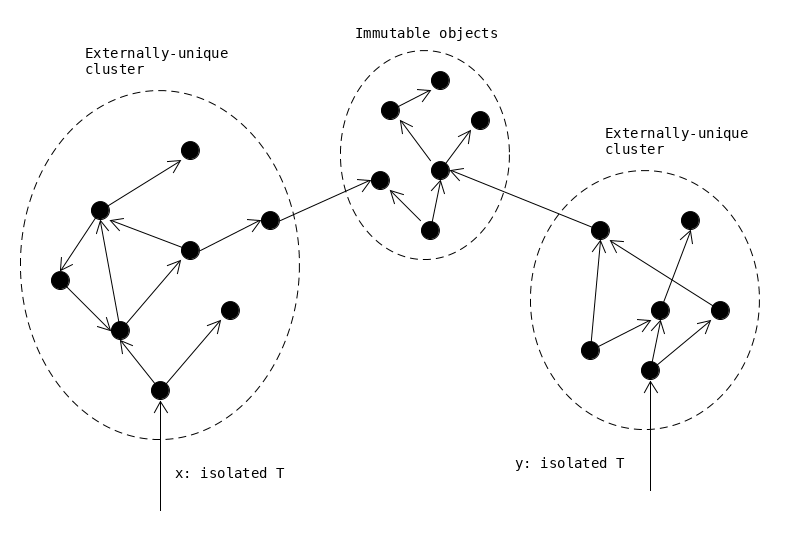
\includegraphics[width=7cm]{uml/isolated-clusters.png}}
	\end{center}
\end{frame}

%%%%%%%%%%%%%%%%%%%%%%%%%%%%%%%%%%%%%%%%%%%%%%%%%%%%%%%%%%%%%%%%%%%%%%%%%%%%

\begin{frame}{Compile-time race-freedom guarantee}
	The paper provides a set of subtyping rules (remember, it's a type
	system). Here are a few:
\end{frame}

\begin{frame}[fragile]{Compile-time race-freedom guarantee}
	\begin{itemize}
	\item it is impossible to acquire a \texttt{writable} reference to
	      an \texttt{immutable} type.
	\end{itemize}
	\begin{lstlisting}
		immutable IntList l = generateRange(0, 100);
		
		// default permission is writable
		IntList mutRef = l; // <- this is forbidden, type error!
		
		mutRef.set(2, -1);
	\end{lstlisting}
\end{frame}

\begin{frame}[fragile]{Compile-time race-freedom guarantee}
	\begin{itemize}
	\item \texttt{isolated} references must be converted before any use,
	      and such a conversion is \textbf{destructive}.
	\end{itemize}
	\begin{lstlisting}
		isolated IntList l = ...;
		
		// update l's permission to writable
		writable IntList l2 = l;
		
		print(l2.get(3)); // ok
		
		l.head = ...; // Type Error!
	\end{lstlisting}
\end{frame}

\begin{frame}[fragile]{Compile-time race-freedom guarantee}
	\begin{itemize}
	\item \texttt{immutable} and \texttt{isolated} references can be
	      recovered under conditions.
	\end{itemize}
	\begin{lstlisting}
		isolated IntBox increment(isolated IntBox b) {
			// implicitly convert b to writable
			b.value++;
			
			// convert b *back* to isolated
			return b;
		}
	\end{lstlisting}
	Is it safe?
	\only<3->{
	\textbf{Yes}: there is only one \texttt{writable} reference to \texttt{b}.}
	\vfill\pause
	\textbf{Note:} The language doesn't allow mutable global variables.
\end{frame}

%%%%%%%%%%%%%%%%%%%%%%%%%%%%%%%%%%%%%%%%%%%%%%%%%%%%%%%%%%%%%%%%%%%%%%%%%%%%

\begin{frame}[fragile]{Compile-time race-freedom guarantee}
	\begin{lstlisting}
		isolated Bar foo(isolated Bar a, isolated Bar b) {
			a.baz = b;
			return b;
		}
	\end{lstlisting}
	\vfill
	\begin{center}
		What about this?
	\end{center}
\end{frame}

\begin{frame}{Compile-time race-freedom guarantee}
	\begin{center}
		\frame{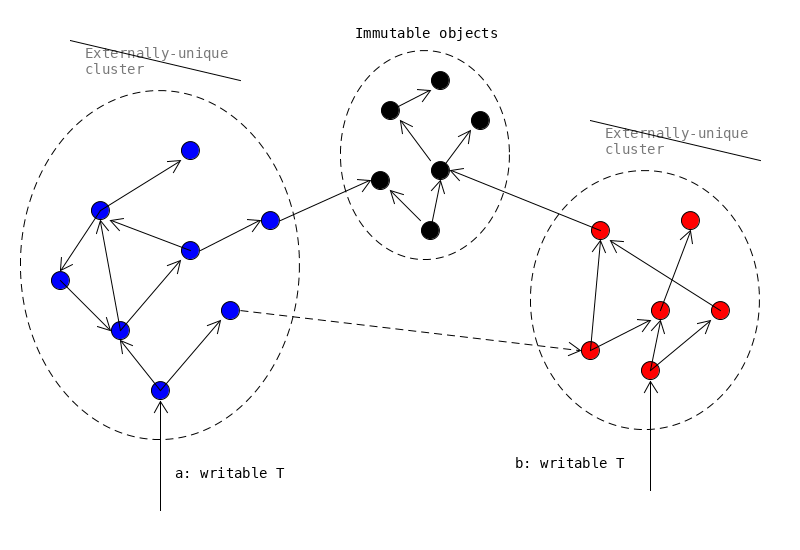
\includegraphics[width=10cm]{uml/quiz-func-2-iso-returns-1-iso-1.png}}
	\end{center}
\end{frame}

\begin{frame}{Compile-time race-freedom guarantee}
	\begin{center}
		\frame{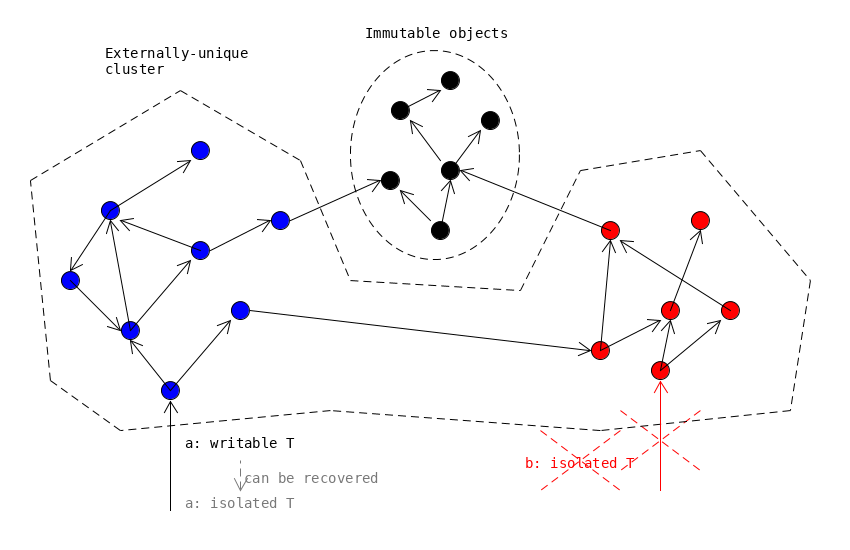
\includegraphics[width=10cm]{uml/quiz-func-2-iso-returns-1-iso-2.png}}
	\end{center}
\end{frame}

\begin{frame}[fragile]{Compile-time race-freedom guarantee}
	The call to \texttt{foo()}:
	\begin{lstlisting}
        isolated IntBox a = ...;
        isolated IntBox b = ...;

        // here, a and b are consumed
        isolated IntBox r = foo(a, b);

        a.x; // Type Error, a has been consumed
        
        // only r is valid now
	\end{lstlisting}
\end{frame}

%%%%%%%%%%%%%%%%%%%%%%%%%%%%%%%%%%%%%%%%%%%%%%%%%%%%%%%%%%%%%%%%%%%%%%%%%%%%

\begin{frame}{Compile-time race-freedom guarantee}
	\begin{center}
		\frame{
\includegraphics[width=7cm]{uml/cool-cool-so-what.png}}
	\end{center}
\end{frame}

%%%%%%%%%%%%%%%%%%%%%%%%%%%%%%%%%%%%%%%%%%%%%%%%%%%%%%%%%%%%%%%%%%%%%%%%%%%%

\begin{frame}{Compile-time race-freedom guarantee}
	\newcommand{\bb}{\only<2->{\color{blue}}}
	\newcommand{\bbb}{\only<4->{\color{blue}}}
	
	The paper presents two forms of parallelism:
	\begin{itemize}
	\item \textbf{Symmetric:} Assuming that {\bb at most one thread}
		  may hold \texttt{writable} references to an object at a given
		  point in time, then while all \texttt{writable} references in
		  a context are {\bb temporarily forgotten}, it becomes
		  {\bb safe to share all read-only or immutable references
		  among multiple threads}, in addition to {\bb partitioning
		  externally-unique clusters between threads}.
	\uncover<3->{
	\item \textbf{Asymmetric:} If all data accessible to a new thread is
		  {\bbb immutable or from externally-unique clusters} which are made
		  {\bbb inaccessible to the spawning thread}, then the new and old
		  threads may run in parallel without interference.
	}
	\end{itemize}
\end{frame}

%%%%%%%%%%%%%%%%%%%%%%%%%%%%%%%%%%%%%%%%%%%%%%%%%%%%%%%%%%%%%%%%%%%%%%%%%%%%

\begin{frame}{Compile-time race-freedom guarantee}
	\begin{center}
		\frame{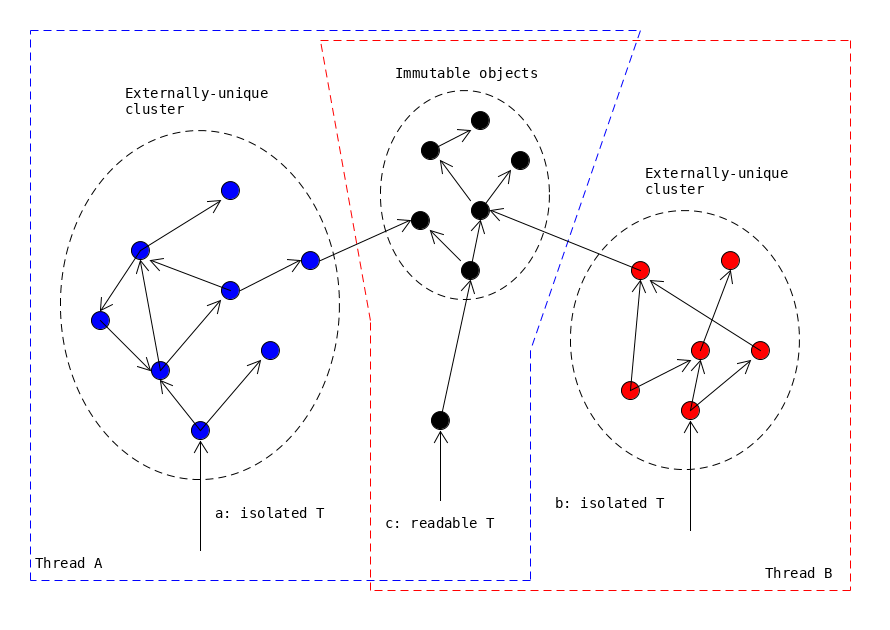
\includegraphics[width=9cm]{uml/par-symmetric.png}}
	\end{center}
	Symmetric parallelism
\end{frame}

\begin{frame}[fragile]{Compile-time race-freedom guarantee}
	\begin{lstlisting}
		x = new Integer(); x.val = 3;
		
		y = x; z = x;
		// y and z are readable aliases of x
		
		a = new Integer(); b = new Integer();
		// a and b are isolated
		
		// frame away writable references (x)
		{ a.val = y.val; } || { b.val = z.val; }
		// get back writable references (x)
		
		x.val = 4;
	\end{lstlisting}
\end{frame}

%%%%%%%%%%%%%%%%%%%%%%%%%%%%%%%%%%%%%%%%%%%%%%%%%%%%%%%%%%%%%%%%%%%%%%%%%%%%

\begin{frame}{Compile-time race-freedom guarantee}
	\begin{center}
		\frame{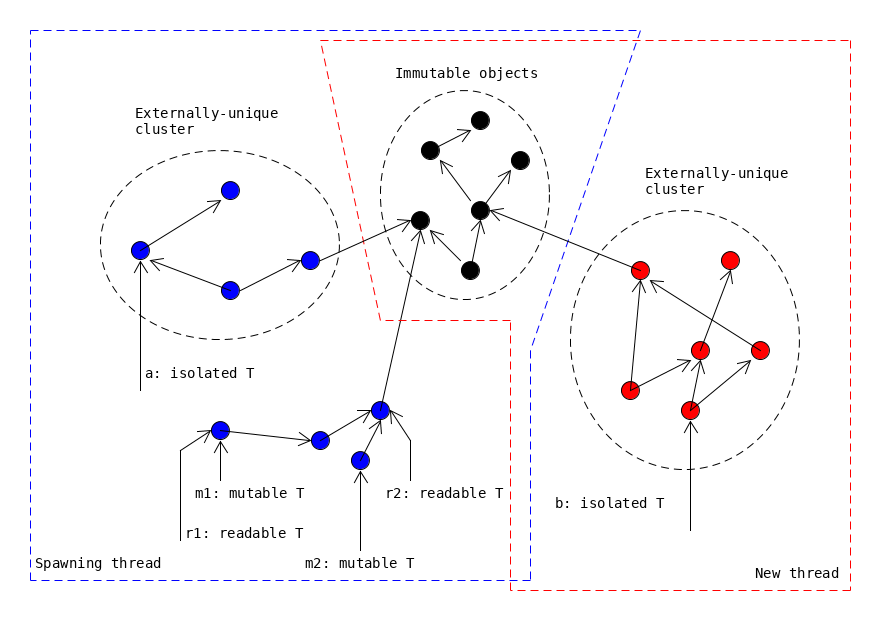
\includegraphics[width=9cm]{uml/par-asymmetric.png}}
	\end{center}
	Asymmetric parallelism
\end{frame}

\begin{frame}[fragile]{Compile-time race-freedom guarantee}
	\begin{lstlisting}
		writable Integer x = ...;
		
		// construct isolated list of isolated integers
		isolated y = new IsolatedIntegerList();
		
		// populate list ...
		
		// Sort in parallel with other work
		{
		    f = new SortFunc();
		    y.map(f);
		} // 1
		|| { x.val = 3; } // 2
	\end{lstlisting}
	1 is the red thread\\
	2 is the blue thread
\end{frame}

\begin{frame}[fragile]{Compile-time race-freedom guarantee}
	\begin{lstlisting}
		writable Integer x = ...;
		isolated y = new IsolatedIntegerList();
		// populate list ...
		
		{
		    f = new SortFunc();
		    y.map(f);
		    y.append(x.val); // Type Error
		}
		|| { x.val = 3; }
	\end{lstlisting}
\end{frame}

%%%%%%%%%%%%%%%%%%%%%%%%%%%%%%%%%%%%%%%%%%%%%%%%%%%%%%%%%%%%%%%%%%%%%%%%%%%%

\begin{frame}{Compile-time race-freedom guarantee}
	Then the paper formalizes all the typing rules. For example:
	\begin{center}
		\frame{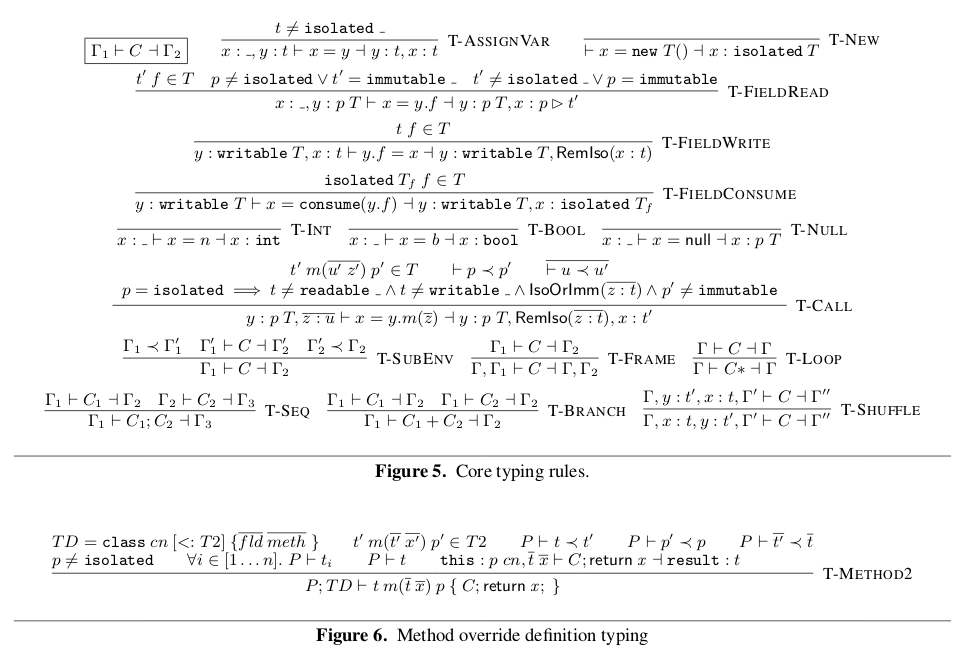
\includegraphics[width=8cm]{img/formulas.png}}
	\end{center}
\end{frame}

%%%%%%%%%%%%%%%%%%%%%%%%%%%%%%%%%%%%%%%%%%%%%%%%%%%%%%%%%%%%%%%%%%%%%%%%%%%%

\begin{frame}{Compile-time race-freedom guarantee}
	But there are only two rules for parallelism:
	\begin{center}
		\frame{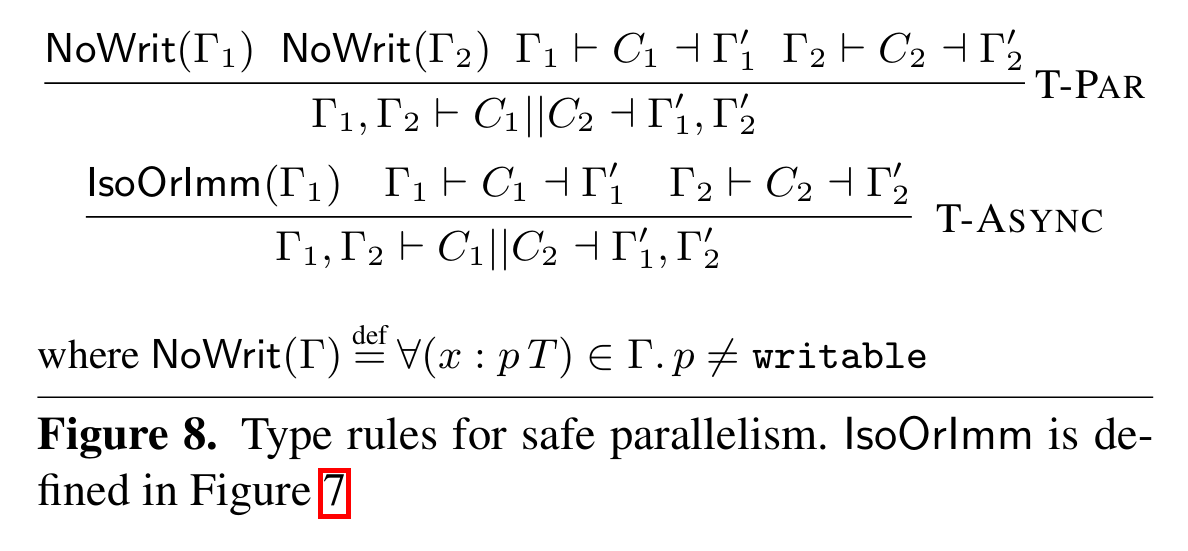
\includegraphics[width=10cm]{img/t-par_t-async.png}}
	\end{center}
\end{frame}

%%%%%%%%%%%%%%%%%%%%%%%%%%%%%%%%%%%%%%%%%%%%%%%%%%%%%%%%%%%%%%%%%%%%%%%%%%%%

\begin{frame}[fragile]{Compile-time race-freedom guarantee}
	So, what is the problem here?
	\begin{lstlisting}
        immutable IntList l = getAgeData();
        writable IntList counters = new IntList();
        
        {
            for (int i = 0; i < l.length / 2; i++)
                counters.inc(l.get(i));
        } || {
            for (int i = l.length / 2; i < l.length; i++)
                counters.inc(l.get(i));
        }
        
        writable Int k = 0;
        writable IntList sorted = new IntList();
        for (int i = 0; i < MAX_AGE; i++)
            for (int j = 0; j < counters.get(i); j++)
                sorted.set(k++, i);
	\end{lstlisting}
\end{frame}

\begin{frame}[fragile]{Compile-time race-freedom guarantee}
	So, what is the problem here?
	\begin{lstlisting}
        immutable IntList l = getAgeData();
        writable IntList counters = new IntList();
        
        {
            for (int i = 0; i < l.length / 2; i++)
                counters.inc(l.get(i)); // Type Error
        } || {
            for (int i = l.length / 2; i < l.length; i++)
                counters.inc(l.get(i)); // Type Error
        }
        
        writable Int k = 0;
        writable IntList sorted = new IntList();
        for (int i = 0; i < MAX_AGE; i++)
            for (int j = 0; j < counters.get(i); j++)
                sorted.set(k++, i);
	\end{lstlisting}
\end{frame}

\begin{frame}[fragile]{Compile-time race-freedom guarantee}
	\begin{lstlisting}
        immutable IntList l = getAgeData();
        isolated IntList c1 = new IntList(), c2 = new IntList();
        
        {
            for (int i = 0; i < l.length / 2; i++)
                c1.inc(l.get(i));
        } || {
            for (int i = l.length / 2; i < l.length; i++)
                c2.inc(l.get(i));
        }
        
        writable Int k = 0;
        writable IntList sorted = new IntList();
        for (int i = 0; i < MAX_AGE; i++)
            for (int j = 0; j < c1.get(i) + c2.get(i); j++)
                sorted.set(k++, i);
	\end{lstlisting}
\end{frame}

%%%%%%%%%%%%%%%%%%%%%%%%%%%%%%%%%%%%%%%%%%%%%%%%%%%%%%%%%%%%%%%%%%%%%%%%%%%%

\begin{frame}{Compile-time race-freedom guarantee}
	\begin{center}
		\frame{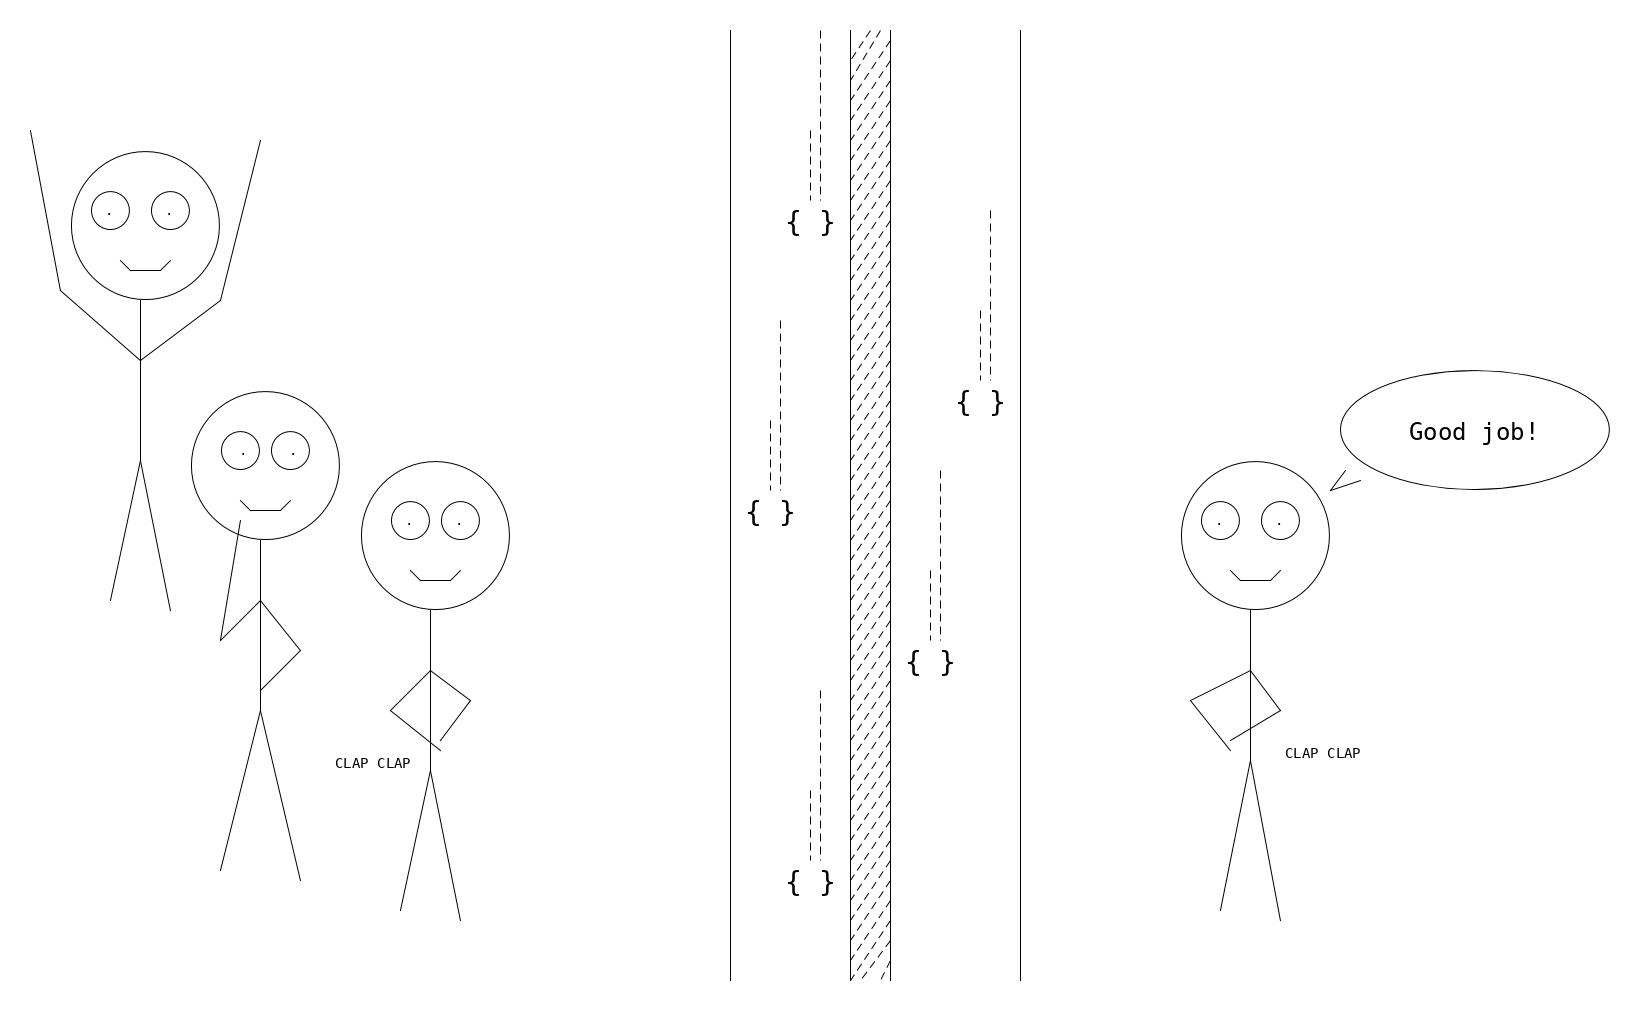
\includegraphics[width=11cm]{uml/bravo.png}}
	\end{center}
\end{frame}

%%%%%%%%%%%%%%%%%%%%%%%%%%%%%%%%%%%%%%%%%%%%%%%%%%%%%%%%%%%%%%%%%%%%%%%%%%%%

\begin{frame}[focus]
	Questions?
\end{frame}

%%%%%%%%%%%%%%%%%%%%%%%%%%%%%%%%%%%%%%%%%%%%%%%%%%%%%%%%%%%%%%%%%%%%%%%%%%%%

\end{document}


























































